\section{The DFiant Language Overview}
\label{sec:dfiant}
DFiant is a Scala library and thus possesses various rich type safe language constructs. DFiant also incorporates unique language semantics that enable dataflow-based hardware description. Throughout this section we elaborate on these constructs and semantics via our running example, a sample filter-accumulator (SFA) that accumulates only \textit{stable} input samples and outputs the accumulated result continuously. An input is considered stable when the last three sample values are distributed within a given standard deviation. The sample input is a 16-bit signed integer and the accumulated output is a 32-bit signed integer. The complete SFA DFiant implementation, its equivalent dataflow graph, and its DFiant-generated VHDL (2008) code are available in \fig{fig:SFADFiant},~\ref{fig:SFADraw}, and~\ref{fig:SFAVHDL}, respectively.


\begin{table*}[t!]
  \centering
  \begin{minipage}[t][23cm][t]{0.46\linewidth}
    \centering
    \begin{minted}[xleftmargin=1.5em,linenos,autogobble,tabsize=2,framesep=1pt, frame=single,fontsize=\fontsize{8}{9}\selectfont]{scala}
      import DFiant._
      
      trait SampleFilterAcc extends DFDesign {
        val stdv      = 1000
        val sample    = DFSInt(16) <> IN
        val acc       = DFSInt(32) <> OUT init 0
        val delta1    = (sample - sample.prev).wc
        val delta2    = (sample - sample.prev(2)).wc
        val usable1   = (delta1 < stdv) && 
                        (delta1 > -stdv)
        val usable2   = (delta2 < stdv) && 
                        (delta2 > -stdv)
        ifdf (usable1 && usable2) {
          acc := acc + sample //acc.prev + sample
        }
      }    
      
      object SFAApp extends App {
        val sfa = new SampleFilterAcc {}
        sfa.compileToVHDL.toFile("sfa.vhd")
      }
    \end{minted}
    \captionof{figure}{SFA DFiant code \\ Some \\ Other}
    \label{fig:SFADFiant}
    \vfill
    \includegraphics[width=\linewidth]{graphics/sfa.pdf}
    \captionof{figure}{SFA dataflow graph \\ hi \\ hello }
		\label{fig:SFADraw}
  \end{minipage}
  \hfill
  \begin{minipage}[t][23cm][t]{0.51\linewidth}
    \centering
    \begin{minted}[xleftmargin=1.5em,linenos,autogobble,tabsize=2,framesep=1pt, frame=single,fontsize=\fontsize{8}{9}\selectfont]{vhdl}
      library ieee;
      use ieee.std_logic_1164.all;
      use ieee.numeric_std.all;
      use work.sfa_pkg.all;
      
      entity sfa is
      port (
        CLK                  : in  std_logic;
        RSTn                 : in  std_logic;
        SAMPLE               : in  signed(15 downto 0);
        ACC                  : out signed(31 downto 0)
      );
      end sfa;
      
      architecture sfa_arch of sfa is
        signal ACC_prev1     : signed(31 downto 0);
        signal SAMPLE_prev1  : signed(15 downto 0);
        signal SAMPLE_prev2  : signed(15 downto 0);
        signal delta1        : signed(16 downto 0);
        signal delta2        : signed(16 downto 0);
        signal delta1_pipe1  : signed(16 downto 0);
        signal delta2_pipe1  : signed(16 downto 0);
        signal usable1       : boolean;
        signal usable2       : boolean;
        signal usable1_pipe1 : boolean;
        signal usable2_pipe1 : boolean;
        signal pipe_stall1   : boolean;
        signal pipe_stall2   : boolean;
      begin
      
      process (CLK, RSTn)
      begin
        if RSTn = '0' then
          ACC_prev1          <= 32d"0";
          pipe_stall1        <= true;     
          pipe_stall2        <= true;
        elsif rising_edge(CLK) then
          ACC_prev1          <= ACC;
          SAMPLE_prev1       <= SAMPLE;  
          SAMPLE_prev2       <= SAMPLE_prev1;
          delta1_pipe1       <= delta1;  
          delta2_pipe1       <= delta2;
          usable1_pipe1      <= usable1; 
          usable2_pipe1      <= usable2;
          pipe_stall1        <= false;     
          pipe_stall2        <= pipe_stall1;
        end if;
      end process;
      
      process (all)
        variable v_ACC       : signed(31 downto 0);
      begin
        v_ACC     := ACC_prev1;
        delta1    <= resize(SAMPLE, 17) - SAMPLE_prev1;
        delta2    <= resize(SAMPLE, 17) - SAMPLE_prev2;
        usable1   <= (delta1_pipe1 < 11d"1000") and 
                     (delta1_pipe1 > -11d"1000");
        usable2   <= (delta2_pipe1 < 11d"1000") and 
                     (delta2_pipe1 > -11d"1000");
        if (usable1_pipe1 and usable2_pipe1) then
          if (not pipe_stall2) then
            v_ACC := v_ACC + SAMPLE_prev2; --SAMPLE_pipe2
          end if;
        end if;
        ACC       <= v_ACC;
      end process;
      
      end sfa_arch;
    \end{minted}
    \captionof{figure}{SFA generated VHDL code}
    \label{fig:SFAVHDL}
  \end{minipage}
\end{table*}

\subsection{Hello DFiant world!}
The SFA DFiant code demonstrates the basics of any DFiant compilation program: it imports the \code{DFiant} library (line 1), creates the top-level design by extending the \code{DFDesign} library trait (lines 3-16), and creates a runnable application that instantiates the top design trait and compiles it into a VHDL file (lines 18-21). 

The SFA design is fairly straightforward. Lines 5 and 6 construct the signed input and output dataflow ports, respectively. Notice that we set an initial 0 value for the accumulated output state (see section ??). Lines 7 and 8 calculate the delta value between the current sample and the previous two samples. The \code{.prev(x)} construct is used to fetch values from the stream history (see section ??). The \code{-} operation, yields a subtractor instance and the \code{.wc} construct is applied to get the a carried result. Lines 9 to 12 compare if the delta values are within the given standard deviation. Finally, lines 13 to 15 conditionally increase the accumulated state, as required. Notice we used \code{acc + sample} and not \code{acc.prev + sample}, but both expression at line 14 are equivalent, since we have an implicit state assignment \code{acc := acc.prev} when an (see section ??). 

The SFA dataflow graph clearly demonstrates the concurrent paths constructed according to the dataflow dependency, even though the code is expressed in a sequential manner. Each application of an arithmetic/logic operator is translated into the appropriate hardware construction and the conditional \code{ifdf} statement is translated into a selector. 

%Note: the shown SFA application uses default configuration for vendor, device, target frequency, etc.  

\subsection{Structural Composition and Generation}

DFiant expands traditional structural composition capabilities by utilizing Scala's object oriented features such as inheritance and polymorphism, as well as finite loops and recursive composition. The hierarchical compositions provide the scope and dependencies for the dataflow variables. The hierarchy itself is transparent to the dataflow graph, as if the entire design is flattened, inlined, and unrolled. Therefore, hierarchies in DFiant are synthesizable, highly reusable, and do not affect the design performance (may affect compilation time). Different composition examples are available in Table~\ref{tbl:Box}.

%\begin{table*}[t]
  \captionof{table}{DFiant Hierarchy Example: Inheritance, Polymorphism, Recursive Composition, and Inlined View}
  \label{tbl:Box}
  \begin{tabular}{|c|c|c|}
    \hline 
    \textbf{Description} & \textbf{DFiant Code} & \textbf{Functional Drawing} \\ 
    \hline
    \begin{minipage}{0.1\textwidth}
      \footnotesize
      \flushleft
      Abstract base class, \code{Box} (defines only an interface)
    \end{minipage} 
    &
    \begin{minipage}{0.48\textwidth}
      \begin{minted}[autogobble,tabsize=2,framesep=1pt,fontsize=\fontsize{8}{8}\selectfont]{scala}
      type DFB = DFUInt[32] //Type alias, to save code space
      abstract class Box(iT: DFB, iB: DFB) { //T=Top, B=Bottom 
        val oT: DFB
        val oB: DFB
      }
      \end{minted}
    \end{minipage} 
    &  
    \begin{minipage}[c][1.5cm]{0.34\textwidth}
      \centering
      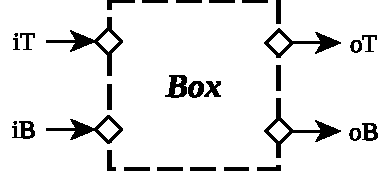
\includegraphics[height=1.3cm]{graphics/Box.pdf}%
    \end{minipage} 
    \\ 
    \hline 
    \begin{minipage}{0.1\textwidth}
      \footnotesize
      \flushleft
      Concrete \code{Box} implementation examples
    \end{minipage} 
    &
    \begin{minipage}{0.48\textwidth}
      \begin{minted}[autogobble,tabsize=2,framesep=1pt,fontsize=\fontsize{8}{8}\selectfont]{scala}
      case class BoxY(iT: DFB, iB: DFB) extends Box(iT, iB) {
        val (oT, oB) = (iT * iT, iT + iB)
      }
      case class BoxE(iT: DFB, iB: DFB) extends Box(iT, iB) {
        val (oT, oB) = (iT + iB, iB)
      }
      \end{minted}
    \end{minipage} 
    &  
    \begin{minipage}[c][1.8cm]{0.34\textwidth}
      \centering
      \includegraphics[height=1.3cm]{graphics/BoxY.pdf}%
      \quad\quad\quad
      \includegraphics[height=1.3cm]{graphics/BoxE.pdf}%
    \end{minipage} 
    \\ 
    \hline
    \begin{minipage}{0.1\textwidth}
      \footnotesize
      \flushleft
      \code{Box123}, an abstract polymorphic composition of three \code{Box} instances
    \end{minipage} 
    &
    \begin{minipage}{0.48\textwidth}
      \begin{minted}[autogobble,tabsize=2,framesep=1pt,fontsize=\fontsize{8}{8}\selectfont]{scala}
      abstract class Box123(iT: DFB, iB: DFB) extends Box(iT, iB){
        def b1Bld(iT: DFB, iB: DFB) : Box
        def b3Bld(iT: DFB, iB: DFB) : Box
        val b1 = b1Bld(iT,     iB)
        val b2 = BoxE(b1.oB,   b1.oT)
        val b3 = b3Bld(b2.oB,  b2.oT)
        val (oT, oB) = (b3.oT, b3.oB)
      }
      \end{minted}
    \end{minipage} 
    &  
    \begin{minipage}[c][2.3cm]{0.34\textwidth}
      \centering
      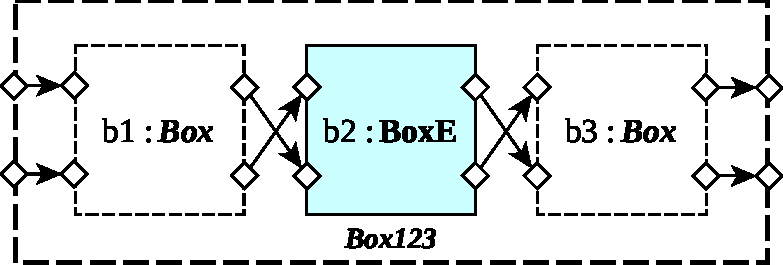
\includegraphics[height=2.1cm]{graphics/Box123.pdf}%
    \end{minipage} 
    \\ 
    \hline
    \begin{minipage}{0.1\textwidth}
      \footnotesize
      \flushleft
      \code{BoxYEE}, a concrete polymorphic composition of three \code{Box} instances \\+\\An inlined view of \code{BoxYEE}
    \end{minipage} 
    &
    \begin{minipage}{0.48\textwidth}
      \begin{minted}[autogobble,tabsize=2,framesep=1pt,fontsize=\fontsize{8}{8}\selectfont]{scala}
      case class BoxYEE(iT: DFB, iB: DFB) extends Box123(iT, iB) {
        def b1Bld(iT: DFB, iB: DFB) = BoxY(iT, iB)
        def b3Bld(iT: DFB, iB: DFB) = BoxE(iT, iB)
      }
      \end{minted}
    \end{minipage} 
    &  
    \begin{minipage}[c][4.6cm]{0.34\textwidth}
      \centering
      \includegraphics[height=2.1cm]{graphics/BoxYEE.pdf} \\
      \vspace{0.1cm}
      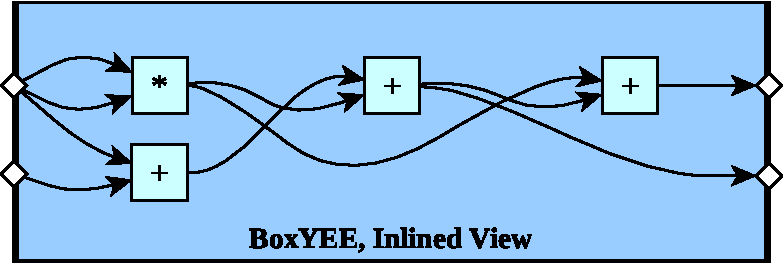
\includegraphics[height=2.1cm]{graphics/BoxYEEInlined.pdf}%
    \end{minipage} 
    \\ 
    \hline
    \begin{minipage}{0.1\textwidth}
      \footnotesize
      \flushleft
      Finite recursive composition example
    \end{minipage} 
    &
    \begin{minipage}{0.48\textwidth}
      \begin{minted}[autogobble,tabsize=2,framesep=1pt,fontsize=\fontsize{8}{8}\selectfont]{scala}
      case class BoxBox(N: Int)(iT: DFB, iB: DFB) 
      extends Box(iT, iB) {
        val b = BoxY(iT, iB)
        val bb : Box = if (N > 0) BoxBox(N - 1)(b.oT, b.oB)
                       else b
        val (oT, oB) = (bb.oT, bb.oB)
      }
      \end{minted}
    \end{minipage} 
    &  
    \begin{minipage}[c][2.3cm]{0.34\textwidth}
      \centering
      \includegraphics[height=2.1cm]{graphics/BoxBox.pdf}%
    \end{minipage} 
    \\ 
    \hline
  \end{tabular} 
\end{table*}


\subsection{IO Ports}
\label{sec:io_ports}
The class \textit{Box} from Table~\ref{tbl:Box} can also be coded as demonstrated in Fig.~\ref{fig:IOBox}. The annotation \code{DFVar $<>$ Dir} controls \textit{DFVar}'s access by encapsulating the variable with the dataflow port class, \code{DFPort}: an \code{IN} port can only be read (immutable), while an \code{OUT} port can only be modified (unreadable). DFiant has implicit conversions in place that selectively converts between \code{DFPort} and \code{DFAny} instances, without breaking mutability rules and type safety. The port annotations match the capabilities of traditional HDLs, and are noticeably absent from HLS languages such as C++. 



\subsection{Dataflow Semantics}
DFiant has a dataflow programming model. Data scheduling order, or \textit{token-flow}, is set by the \textit{data dependency}. Essentially, the DFiant semantics schedules all independent dataflow expressions concurrently, while dependent operations are synthesized into a guarded FIFO-styled pipeline. Dataflow branches are implicitly forked and joined. Unused nodes, semantically, always consume tokens, and are discarded during compilation. We observe the DFiant \code{f} implementation as follows:

\begin{enumerate}
  \item All expressions are dataflow variable declarations.
  \item Concurrency is implicit, and \code{f} is coded intuitively, in a sequential manner, since dataflow dependency is oblivious to statement order. 
  \item All scheduling is implicitly guarded by its dependencies. For example, \code{a} is forked into both \code{b} and \code{c} operations, while \code{c} joins branches from \code{a} and \code{b}.
  It is impossible to read an invalid result or an old result (without extending semantics further).
  \item DFiant semantics are intuitive: data is consumed only when it is ready and can be accepted by all receiving nodes, while back-pressure prevents data loss. 
\end{enumerate} 

%The basic DFiant types are DFBits and DFBool
%Each dataflow type points to a static bits vector
%As can be seen from Related Work, HLS "LO TAFAS". Fig. \ref{boxy}
%WE believe one of the primary reasons is that missing features of RTL
%In this section we will cover the RTL features of RTL and how they handled in DFiant's abstractions
%Bring type driven development into hardware design.
%Need inheritance tree.
%Interactions with scala types


\subsection{Bit-Accurate Operations, Type Inference, and Data Structures}
All DFiant's dataflow types are bit-accurate and structurally static, with their bit-width set upon construction (e.g., \code{DFBits[5]} is a 5-bit vector). Operations between dataflow variables produce a bit-accurate result with the proper type inference. For example, an addition between an unsigned 5-bit variable (\code{DFUInt[5]}) and a signed 10-bit variable (\code{DFSInt[10]}) produces an adder that can be implicitly converted to a 10-bit signed variable, if carry is not required, or an 11-bit signed variable by explicitly invoking \code{.wc} from the addition.

DFiant also allows operations between dataflow types and their corresponding Scala numeric types, by treating the Scala numeric types as constants (e.g., addition between \code{DFSInt} and \code{Integer} variables). A constant in the dataflow graph is a node that can produce infinite tokens of the same value.   

\subsection{Mutability}
\label{sec:mutability}
DFiant supports dataflow variables mutability via the \code{:=} operator. Do not confuse with Scala-level mutability which is enabled by using \code{var} instead of \code{val}. Each dataflow class has two variations: an immutable class, which inherits from \code{DFAny\textbf{Val}} and a mutable class, which inherits from \code{DFAny\textbf{Var}} and accepts \code{:=}. The difference between the types enforces an immutable right-hand-side (RHS), where required, and a mutable variable creation. Consider, for instance, the DFiant implementation of \code{g} in Table \ref{tbl:StateExDefImpl}: \code{a} is immutable because it is a RHS addition between the dataflow variable \code{i} and a literal value \code{5}. Contrarily, \code{c} is mutable, since it is a dataflow variable constructor (\code{.init} constructs a new initialized variable, while preserving the mutability trait). 

Fig.~\ref{fig:Inherit} demonstrates a dual class definition for every type  (immutable and mutable). The naming convention helps to reason about the mutability. For example, \code{DFBits} and \code{DFBits.Var} are immutable and mutable classes, respectively. Constructing a new variable via \code{DFBits} (e.g, \code{val a = DFBits[5]}) returns the mutable \code{DFBits.Var[5]}. Usually, we either receive or return an immutable type, hence we do not require annotating a type with its mutable variation. In cases where we want to return a mutable type, we annotate it as an output port (see Section~\ref{sec:io_ports}).

%DFiant's code safety is enforced by maintaining the 'DF-mutability' trait while aliasing (accepting the ':=' operator). This means that an alias of a \textbf{Var}, is still a \textbf{Var}, and can be assigned, while an alias of a \textbf{Val} cannot. This concept is illustrated in ???, and further explained in ???:




\subsection{Bit Aliasing and Casting}
Aliasing in DFiant enables referencing a part of a dataflow variable, by invoking \code{.bits(hiIdx, loIdx)}, which creates a bits vector alias that references the original variable at the given index parameters. Every change of a dataflow variable affects its alias and vice versa (similar to VHDL's signal aliasing). Since this function also casts the variable as \code{DFBits}, this feature is used as a raw-data cast between different dataflow types. Aliasing of an alias is also possible, while maintaining relative bits indexing. Aliasing preserves the mutability trait: an alias of an immutable variable is immutable, while an alias of a mutable variable is mutable. 


Fig.~\ref{fig:Aliasing} demonstrates aliasing code and its effect on the contents of a dataflow variable (\code{bits128}). Each line code does as follows:
\begin{enumerate}
  \item Constructs a new 128-bit vector, \code{bits128}, and clears it.
  \item Creates a new alias, \code{alias64}, which references the most significant 64 bits of \code{bits128}. Since \code{bits128} is a \code{DFBits} variable, there is no need to invoke \code{.bits()}, and we can apply the required indexes directly.
  \item Creates a new alias, \code{alias32}, which references the least significant 32 bits of \code{alias64}, which reference bits 64 to 95 of \code{bits128}.
  \item Constructs a new double precision floating point dataflow variable, \code{dbl}, and initialize its value as \code{1.0} (hexadecimal value of \code{0x3FF00...0}).
  \item Modifies the least significant byte of \code{dbl}.
  \item Sets the most significant bit of \code{bits128}.
  \item Assigns \code{dbl} to the least significant 64 bits of \code{bits128} through casting. All the bits of \code{dbl} are selected because \code{.bits()} is invoked without index parameters.
  \item Modifies a byte of \code{bits128}.
  
\end{enumerate}

%\begin{figure}[h]
%  \centering
%  \begin{minipage}[b][3cm][b]{0.57\linewidth}
%    \vfill
%    \begin{minted}[xleftmargin=1.5em,linenos,autogobble,tabsize=2,framesep=1pt, frame=single,fontsize=\fontsize{8}{8}\selectfont]{scala}
%      val bits128 = DFBits[128] := 0
%      val alias64 = bits128(127, 64)
%      val alias32 = alias64(31, 0)
%      val dbl = DFDouble := 1.0
%      dbl.bits(7,0) := 0x28
%      bits128(127) := 1
%      bits128(63, 0) := dbl.bits()
%      alias32(16, 8) := 0x57		    
%    \end{minted}
%    \vfill
%    \subcaption{DFiant code}
%  \end{minipage}%
%  \hfill
%  \begin{minipage}[b][3cm][b]{0.42\linewidth}
%    \centering
%    \vfill
%		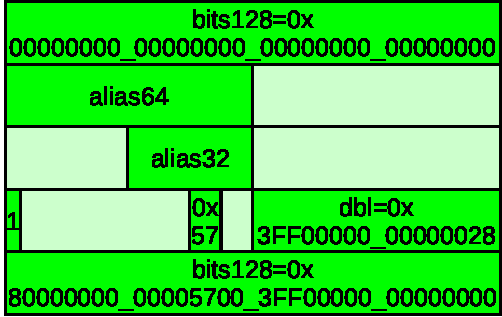
\includegraphics[width=\linewidth]{graphics/Aliasing.pdf} 
%    \vfill
%    \subcaption{Contents of \code{bits128}}
%  \end{minipage}
%  \captionof{figure}{Bit aliasing and casting example}
%  \label{fig:Aliasing}
%\end{figure}


\subsection{How much code we save vs VHDL}
Explicitly saving history for sample
Thanks to type inference, no need to declare types for internal values.
No need to extend the a value to get a carried result.
No need to create explicit pipeline (which also changed according to the target device).
No need to explicitly create stall logic.

\subsection{Brainstorming}
We are replacing concepts of register and wire to state and stateless. This is key difference between dataflow and RTL HDLs. Dataflow assumes there is always a history, in every dataflow value. So we can access the history, yet call it stateless.


%\begin{figure}[h]
%  \centering
%  \begin{minipage}{0.4\linewidth}
%  \begin{minted}[autogobble,tabsize=2,framesep=1pt, frame=single,fontsize=\fontsize{8}{8}\selectfont]{scala}
%  abstract class Box() { 
%    val iT: DFB <> IN
%    val iB: DFB <> IN
%    val oT: DFB <> OUT
%    val oB: DFB <> OUT
%  }
%  \end{minted}
%  \end{minipage}
%  \captionof{figure}{IO port annotation DFiant code example}
%  \label{fig:IOBox}
%\end{figure}



%+ C has no clear input/output notation. Input array and output array are the same.
%
%+ IDE: Intellisense, error highlighting, code completion, watches, println.
%+ Unified compilation
%+ Complete project build with the IDE. Compile results.
%Yes abstract away pipelining. No to scheduling control.
%
%Features we don't want
%simulations constructs.
%separate constraints file.
%
%VHDL Possible race conditions.
%
%
%+Include a summary table of RTL feature abstraction and how their are defined in DFiant.

